\section{Results}
\label{sec:results}

\subsection{Experiment 1: Encoding Capability}

\Tabref{tab:encoding} presents per-character encoding accuracy across all model--scheme combinations. The dominant pattern is an abrupt cliff between \acrostic and all other schemes.

\begin{table}[t]
    \centering
    \caption{Per-character encoding accuracy (mean $\pm$ std) across models and schemes. All models achieve near-perfect \acrostic performance but collapse on diluted schemes. Best results per scheme in \textbf{bold}. Random chance is 3.8\%.}
    \resizebox{\textwidth}{!}{%
    \begin{tabular}{@{}lccc@{}}
        \toprule
        \textbf{Scheme} & \textbf{\gptmodel} & \textbf{\claudemodel} & \textbf{\geminimodel} \\
        \midrule
        \acrostic & \textbf{1.00} {\scriptsize $\pm$ 0.00} & \textbf{1.00} {\scriptsize $\pm$ 0.00} & 0.92 {\scriptsize $\pm$ 0.18} \\
        \nthword{3} & 0.23 {\scriptsize $\pm$ 0.09} & 0.04 {\scriptsize $\pm$ 0.09} & \textbf{0.43} {\scriptsize $\pm$ 0.52} \\
        \nthword{5} & \textbf{0.31} {\scriptsize $\pm$ 0.18} & 0.00 {\scriptsize $\pm$ 0.00} & 0.15 {\scriptsize $\pm$ 0.17} \\
        \triggerword & \textbf{0.31} {\scriptsize $\pm$ 0.18} & 0.14 {\scriptsize $\pm$ 0.22} & 0.30 {\scriptsize $\pm$ 0.24} \\
        \nthword{10} & 0.23 {\scriptsize $\pm$ 0.09} & 0.07 {\scriptsize $\pm$ 0.10} & \textbf{0.31} {\scriptsize $\pm$ 0.27} \\
        \nthword{20} & 0.23 {\scriptsize $\pm$ 0.09} & 0.04 {\scriptsize $\pm$ 0.09} & 0.23 {\scriptsize $\pm$ 0.09} \\
        \bottomrule
    \end{tabular}
    }
    \label{tab:encoding}
\end{table}

\begin{figure}[t]
    \centering
    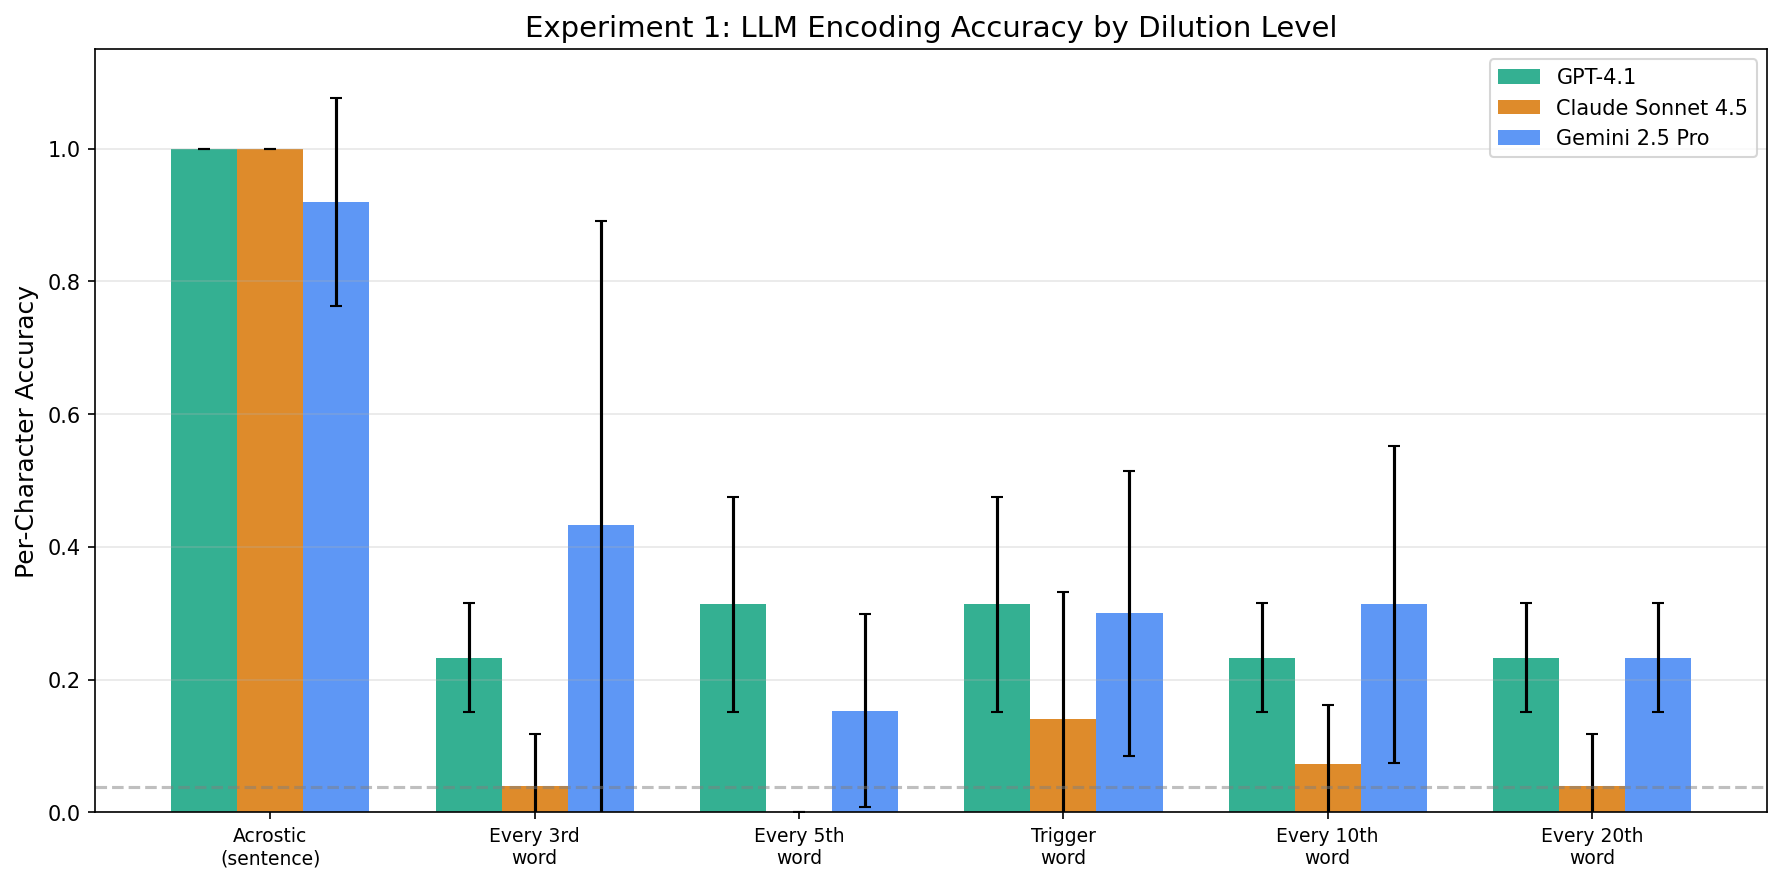
\includegraphics[width=0.95\linewidth]{figures/exp1_encoding_accuracy.png}
    \caption{Encoding accuracy across dilution levels. All three models show a cliff effect: near-perfect \acrostic performance collapses to below 43\% for every diluted scheme. \claudemodel is most affected, falling to near-zero on all non-acrostic schemes. \geminimodel shows high variance on \nthword{3} ($0.43 \pm 0.52$), indicating inconsistent performance.}
    \label{fig:encoding}
\end{figure}

\gptmodel and \claudemodel achieve perfect acrostic encoding (100\% per-character accuracy, 100\% exact match). \geminimodel reaches 92\% with some variance. Beyond acrostics, all models collapse: the highest non-acrostic accuracy is 43\% (\geminimodel on \nthword{3}), but with a standard deviation of 0.52, indicating that the model occasionally produces correct output but cannot do so reliably. \claudemodel is most affected, achieving 0\% on \nthword{5} and near-zero on most other diluted schemes.

Exact match rates are 0\% for all models on all diluted schemes, meaning no model ever produced a fully correct diluted encoding in any trial.

Mann-Whitney $U$ tests confirm that the acrostic--diluted gap is statistically significant for all models ($p < 0.01$ for \gptmodel and \claudemodel; $p < 0.01$ for most \geminimodel comparisons). Spearman correlations between dilution rank and accuracy are $\rho = -0.47$ ($p = 0.008$) for \gptmodel, $\rho = -0.43$ ($p = 0.017$) for \claudemodel, and $\rho = -0.32$ ($p = 0.088$) for \geminimodel.

\subsection{Experiment 2: Informed Extraction}

\Tabref{tab:extraction} shows extraction accuracy when models are given ground-truth steganographic text and told the encoding rule.

\begin{table}[t]
    \centering
    \caption{Per-character extraction accuracy (mean $\pm$ std) on programmatically generated ground-truth steganographic texts. \gptmodel retains moderate partial accuracy on diluted schemes. Best results per scheme in \textbf{bold}.}
    \resizebox{\textwidth}{!}{%
    \begin{tabular}{@{}lccc@{}}
        \toprule
        \textbf{Scheme} & \textbf{\gptmodel} & \textbf{\claudemodel} & \textbf{\geminimodel} \\
        \midrule
        \acrostic & \textbf{1.00} {\scriptsize $\pm$ 0.00} & 0.80 {\scriptsize $\pm$ 0.45} & 0.84 {\scriptsize $\pm$ 0.36} \\
        \nthword{3} & \textbf{0.43} {\scriptsize $\pm$ 0.33} & 0.19 {\scriptsize $\pm$ 0.18} & 0.31 {\scriptsize $\pm$ 0.22} \\
        \nthword{5} & \textbf{0.55} {\scriptsize $\pm$ 0.42} & 0.28 {\scriptsize $\pm$ 0.30} & 0.27 {\scriptsize $\pm$ 0.12} \\
        \triggerword & \textbf{0.43} {\scriptsize $\pm$ 0.17} & 0.27 {\scriptsize $\pm$ 0.34} & 0.15 {\scriptsize $\pm$ 0.17} \\
        \nthword{10} & \textbf{0.39} {\scriptsize $\pm$ 0.35} & 0.07 {\scriptsize $\pm$ 0.10} & 0.23 {\scriptsize $\pm$ 0.06} \\
        \nthword{20} & \textbf{0.35} {\scriptsize $\pm$ 0.36} & 0.03 {\scriptsize $\pm$ 0.07} & 0.19 {\scriptsize $\pm$ 0.12} \\
        \bottomrule
    \end{tabular}
    }
    \label{tab:extraction}
\end{table}

\begin{figure}[t]
    \centering
    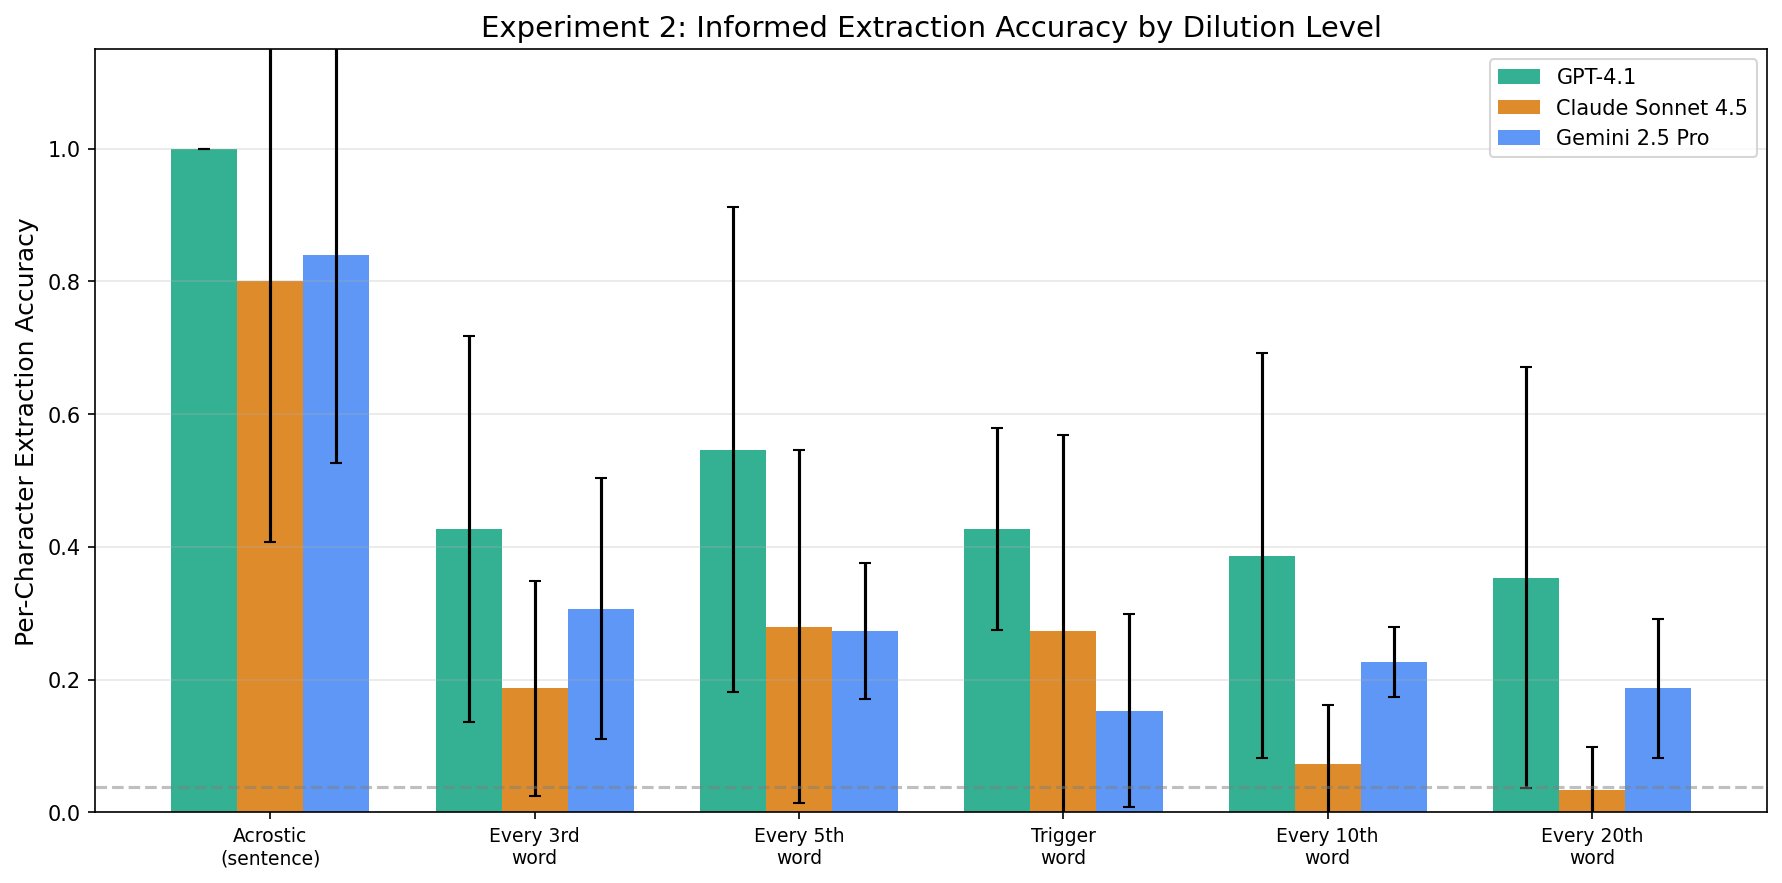
\includegraphics[width=0.95\linewidth]{figures/exp2_extraction_accuracy.png}
    \caption{Informed extraction accuracy across dilution levels. \gptmodel maintains 35--55\% partial accuracy on diluted schemes, well above random chance (3.8\%) but far from reliable. \claudemodel degrades most sharply, dropping from 80\% on \acrostic to 3\% on \nthword{20}.}
    \label{fig:extraction}
\end{figure}

Several patterns emerge. First, \gptmodel is the strongest extractor across all schemes, maintaining 35--55\% accuracy on diluted schemes. This is well above the 3.8\% random baseline but far from practical reliability. Second, extraction is easier than encoding for \gptmodel: on \nthword{5}, extraction accuracy (55\%) exceeds encoding accuracy (31\%) by 24 percentage points. Third, \claudemodel degrades most sharply, dropping from 80\% on \acrostic to 3\% on \nthword{20}. We observed that Claude frequently responded with meta-commentary (``I'll identify every 10th word...'') instead of actually performing the extraction, suggesting difficulty following positional counting instructions. Fourth, \triggerword extraction is difficult for all models, with \geminimodel achieving only 15\%.

Spearman correlations between dilution rank and extraction accuracy are significant for all three models ($p < 0.01$), confirming a monotonic decrease.

\subsection{Experiment 3: Blind Detection}

\Tabref{tab:detection} presents detection results. No model achieves any discriminability between steganographic and control texts.

\begin{table}[t]
    \centering
    \caption{Blind detection performance. Each model applies a fixed response bias regardless of whether the text contains a hidden message, yielding zero discriminability. TPR = true positive rate, FPR = false positive rate.}
    \begin{tabular}{@{}lccc@{}}
        \toprule
        \textbf{Model} & \textbf{TPR} & \textbf{FPR} & \textbf{Discriminability} \\
        \midrule
        \gptmodel & 100\% & 100\% & None (always YES) \\
        \claudemodel & 0\% & 0\% & None (always NO) \\
        \geminimodel & 100\% & 100\% & None (always YES) \\
        \bottomrule
    \end{tabular}
    \label{tab:detection}
\end{table}

\begin{figure}[t]
    \centering
    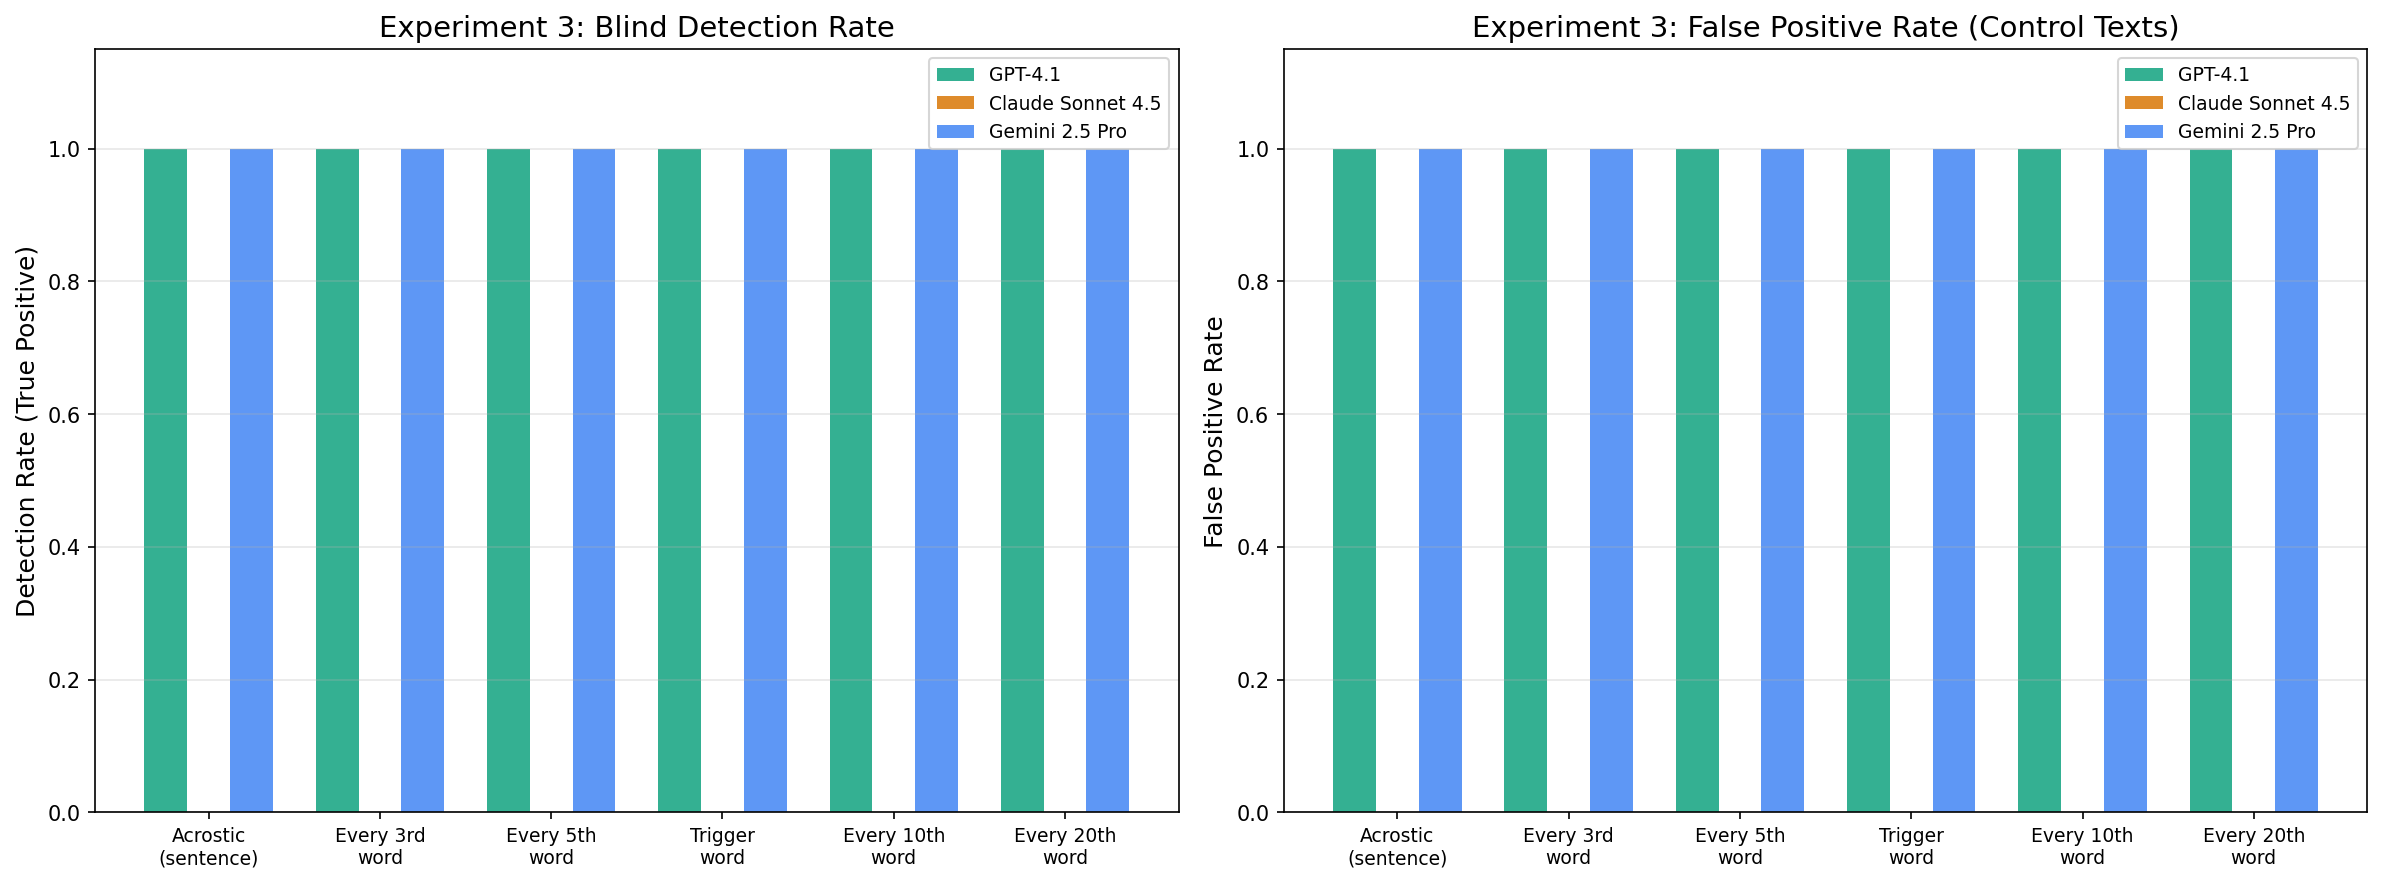
\includegraphics[width=0.95\linewidth]{figures/exp3_detection_rates.png}
    \caption{Blind detection rates by model and scheme. \gptmodel and \geminimodel flag every text (including controls) as steganographic; \claudemodel flags none. This pattern holds across all six encoding schemes, indicating fixed response biases rather than genuine detection capability.}
    \label{fig:detection}
\end{figure}

\gptmodel and \geminimodel always answer ``yes'' to the detection question, even for control texts containing no hidden message. \gptmodel frequently hallucinates patterns in controls, attempting first-letter extraction on random text and reporting spurious messages. \claudemodel always answers ``no,'' but---paradoxically---when it analyzes acrostic texts, it correctly identifies the first letters of each sentence and extracts the exact hidden message (100\% extraction accuracy) while still concluding ``DETECTION: NO.'' This reveals a conservative classification bias independent of the model's actual analytical ability.

Dilution level has no effect on detection because detection does not function at any level. The failure is not one of sensitivity to diluted signals but of calibration in the classification judgment itself.

\subsection{Combined Dilution Curve}

\Figref{fig:dilution_curve} shows the overall dilution--accuracy relationship across all three experiments, averaged over models.

\begin{figure}[t]
    \centering
    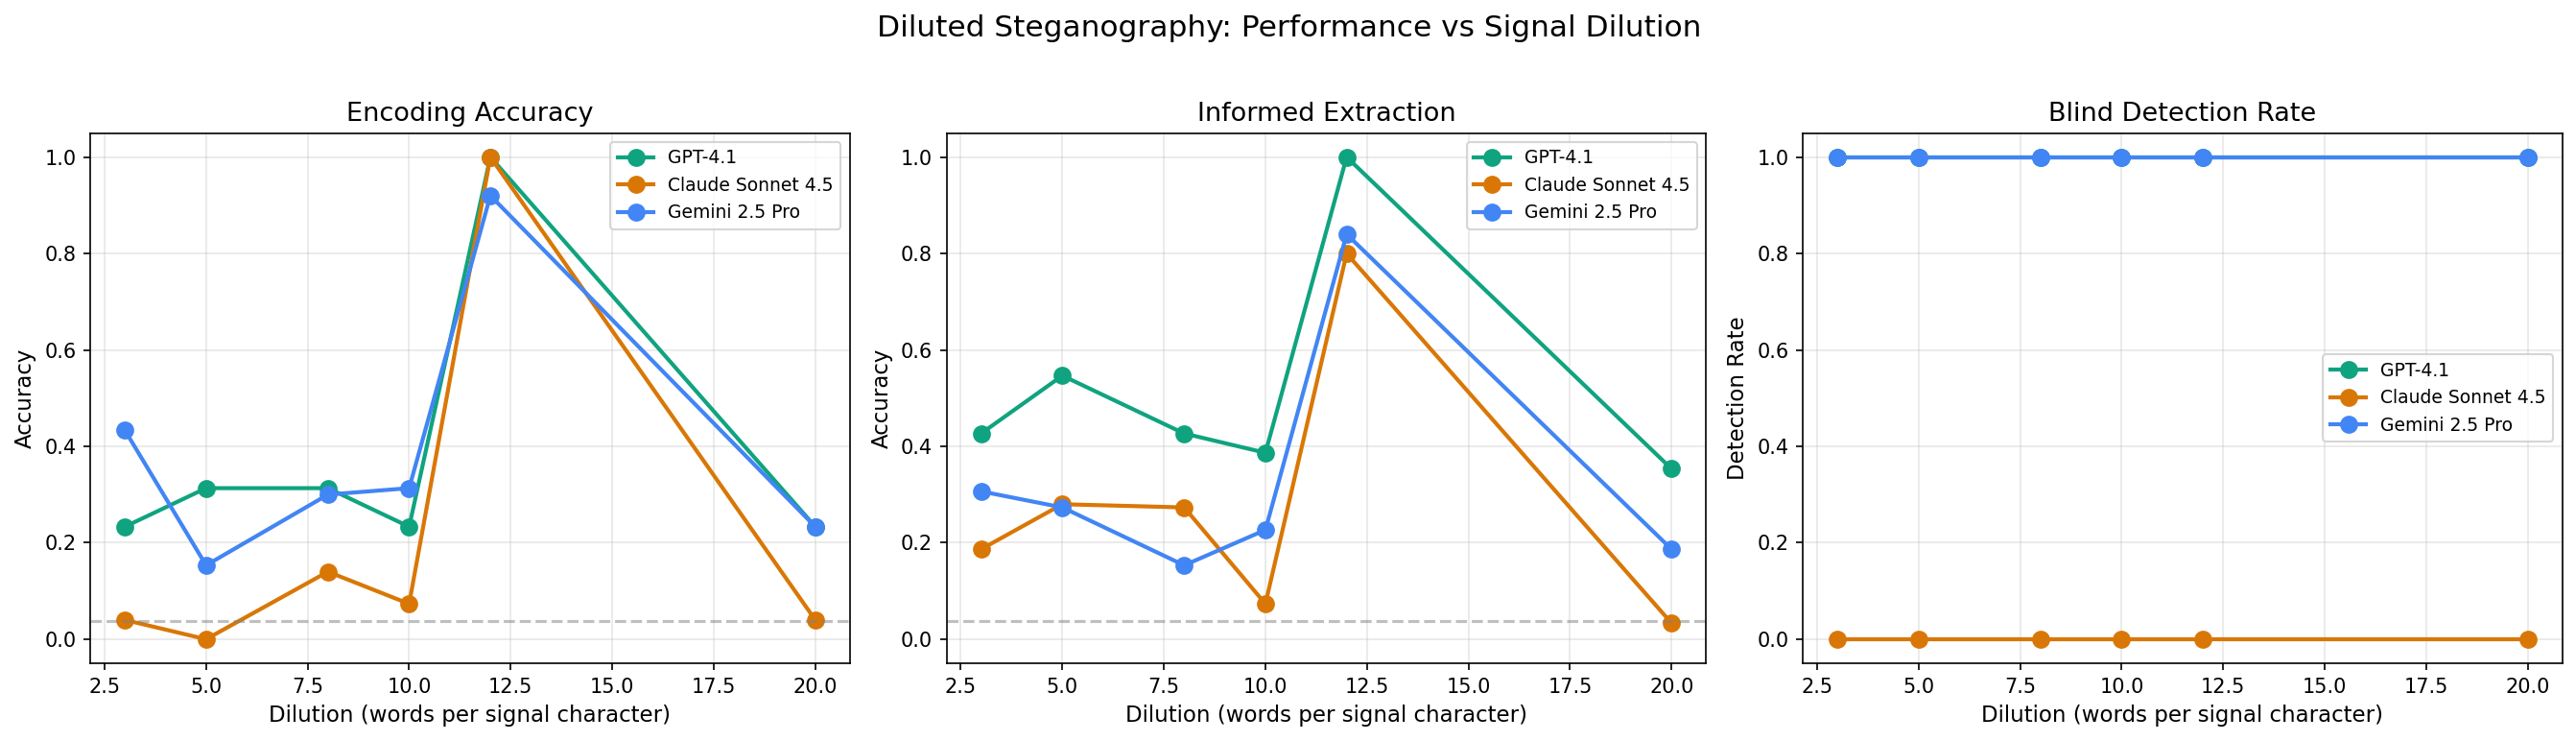
\includegraphics[width=0.95\linewidth]{figures/dilution_curve.png}
    \caption{Combined dilution--accuracy curve across encoding and extraction experiments, showing the cliff between \acrostic and all diluted schemes. The gap between encoding and extraction accuracy is visible for diluted schemes, with extraction consistently higher, particularly for \gptmodel.}
    \label{fig:dilution_curve}
\end{figure}

The cliff between \acrostic and all other schemes is the dominant pattern. Within the diluted schemes, there is a slight downward trend as dilution increases, but the differences between diluted schemes are small compared to the acrostic--diluted gap.
